

\section{The Cumulus System}
\label{sec:architecture}


\subsection{Architecture}


\begin{figure}
\hspace{-3mm}
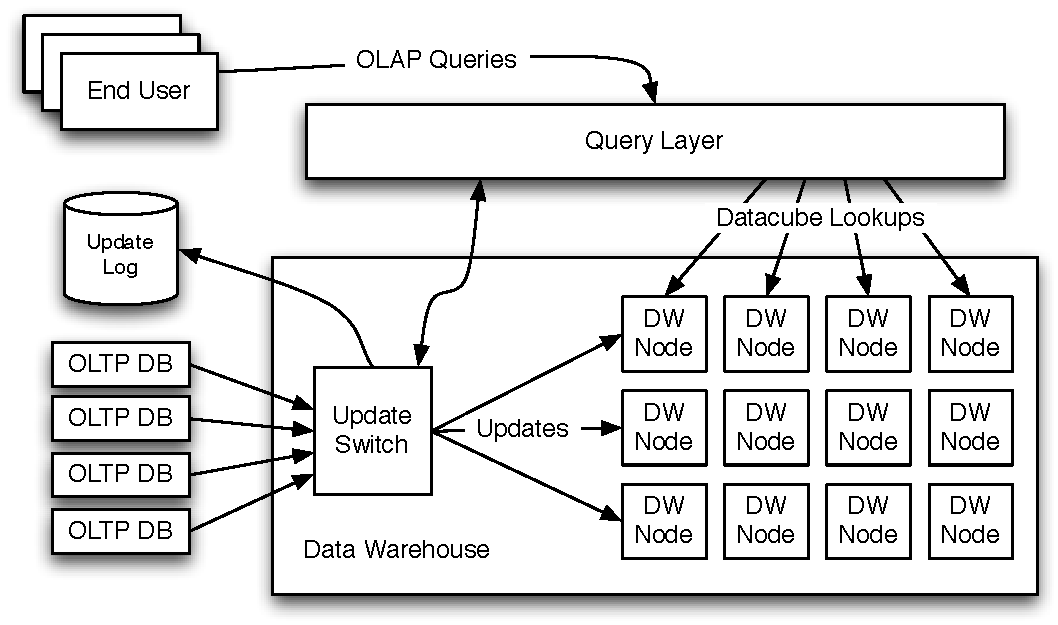
\includegraphics[width=3.4in]{images/Architecture.pdf}

\vspace{-4mm}

\caption{Cumulus' architecture.}
\label{fig:arch}
\end{figure}


Cumulus consists of three components: the compiler,
a {\em runtime}, and a {\em query layer}.
A diagram of this architecture is presented in Figure \ref{fig:arch}.

The compiler, which was discussed in the
previous section, translates SQL aggregation queries
into message passing programs that are executed by the runtime system.

The runtime accepts updates -- insertions and deletes of tuples --
at a coordinator node called the \textit{Switch}, which delegates
update work to a number of data storage and query processing nodes, or
\textit{DW Nodes}.
The maps suggested by the compiler -- and maintained by the M3 program --
are partitioned across the DW Nodes to keep network traffic to a minimum.  
The switch does not store any map data, but manages
the information about data placement (how maps are partitioned and which
partitions are located on which nodes).

The runtime is designed to implement exact online aggregation, and
we conceive it to be used for main-memory OLAP.
The query layer accepts roll-up/drill-down/slice/dice queries,
instructs the Switch to have the DW Nodes send a consistent version of
the relevant data to the querying node (the user's machine),
collects the result chunks there, and
finalizes the query answer
in a client-side API that runs on the user machine.

Our architecture supports the compilation of pre-aggrega\-tors close to the
OLTP database that reduce the load on Cumulus. For example, if sums of revenues
are to be computed, the revenues of batches of LineOrder tuples agreeing
on relevant join and group-by columns can be pre-aggregated close to the OLTP database and only this reduced workload of preaggregated tuples is sent to the Switch.

We generally assume that the data is persistent in the OLTP databases.
However, Cumulus is also able to
log the update stream arriving at the Switch and replay it from the
log later to recreate the data warehouse in main memory.
We could also log the map states using techniques as surveyed in
\cite{DBLP:journals/pvldb/SallesCSDGKW09}
for faster recovery, but this is currently not done.



\subsection{Data Placement}


The Switch maintains information how map data is partitioned across
DW Nodes. In the most general case, this would be a function
that maps a tuple update and a statement (id) from the M3 program to
a record that identifies, for each map access of the statement,
which DW Nodes store any relevant data for executing this
statement.
%
In the current prototype of Cumulus, maps are partitioned along
dimensional axes, akin to the partitioning done in grid files\cite{318586}.


\begin{example}\em
\label{ex:switch_msg}
Consider the M3 program of Example~\ref{ex:ssb}.
Assume there are nodes $N_1$ to $N_5$,
which store the following map partitions:
\begin{eqnarray*}
N_1 &:& mPL[*, \mbox{odd years}] \\
N_2 &:& mPL[*, \mbox{even years}], mDL[*, \mbox{green parts}] \\ 
N_3 &:& mDL[*, \mbox{red parts}] \\ 
N_4 &:& m[*, \mbox{odd years}] \\
N_5 &:& m[*, \mbox{even years}]
\end{eqnarray*}

Suppose {\tt on insert into Date($d_1$, 2005)} is triggered.
The trigger consists of only one statement,
{\tt mPL[datekey, year] += 1}, where datekey and year are instantiated
with $d_1$ and 2005, respectively. Since 2005 is odd,
the map values to be written are located on node $N_1$.
The statement contains no map values to be {\em read}.

For {\tt on insert into LineOrder($d_1$, $p_1$, $500$)},
there is one statement, which reads from $mPL$ and $mDL$ and writes to $m$.
The tuple ($d_1$, $p_1$, $500$)
does not provide useful information for restricting the nodes to be contacted
in this case.
Values of $m$ may be located on $N_4$ and $N_5$, values of $mPL$ may be
located on $N_1$ and $N_2$, and values of $mDL$ may be located on $N_2$ and
$N_3$.
\punto
\end{example}


\nop{
\begin{figure}
\begin{center}
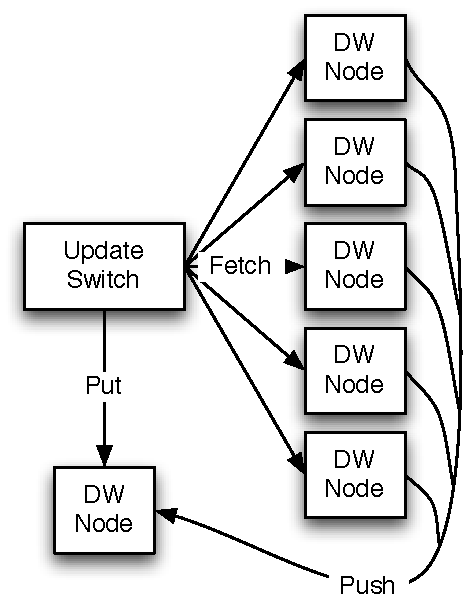
\includegraphics[width=1.5in]{images/UpdateStep.pdf}
\caption{Information flow during one map update.}
\label{fig:updatestep}
\end{center}
\end{figure}
} % end nop


\subsection{Update Protocol}


On an {\em update} (an insertion or deletion of a tuple
$\vec{x}\vec{y}$), an M3 program processes a set of statements of the form
\[
\mbox{{\tt foreach $\vec{z}$ do} $m[\vec{x}\vec{z}]$ += $t$
~~~~~or~~~~~ $m[\vec{x}]$ += $t$}
\]
in {\em arbitrary}\/ order.
%
Each update has a sequence number identifying it. All messages sent by the
Switch contain this update sequence number.

For a given statement, the Switch proceeds as follows.
It composes a set of messages parametrized on $\vec{x}\vec{y}$ and
dispatches them to the DW Nodes.
DW Nodes being read from are sent FETCH requests, which leads them to forward
PUSH messages containing the data read
to the appropriate writers. The writers are also
informed of their role by the Switch through PUT messages.

The update corresponding to an M3 statement is handled by the subset of
nodes that store partitions of the map being written to.  Each node
handles updates only for those partitions it stores locally. The Switch
uses the partition table to only contact readers who may store relevant information and writers who may have updates to do. 


As stated already, the nodes receiving a FETCH request perform the
requested reads and send their responses to the PUT nodes (the writers)
in a PUSH message.
The writers buffer received PUSH messages. For each write task to be
done, they receive a PUT message from the Switch which instructs them
what write to perform and which readers to expect PUSH messages from.
Readers who have received a FETCH message from the Switch always
send a PUSH message to the writers that were
identified by the Switch in the FETCH
message: If a reader has no relevant data, it sends an empty PUSH message to
the writer to allow it to move on.
This allows the writer to know when all necessary PUSH messages have been
received and the write can be carried out.

%An illustration of the complete message-passing process is given
%in Figure \ref{fig:updatestep}.  


\begin{figure}
\begin{center}
\begin{tabular}{l|r@{~}l}
to node & & message \\
\hline
$N_1$ & FETCH($t$, $s$, & push mPL[$d_1$, *] to $\{N_4\}$) \\[.7ex]
$N_2$ & FETCH($t$, $s$, & push mPL[$d_1$, *] to $\{N_5\}$ and \\
      &                 & push mDL[$p_1$, *] to $\{N_4, N_5\}$) \\[.7ex]
$N_3$ & FETCH($t$, $s$, & push mDL[$p_1$, *] to $\{N_4, N_5\}$) \\[.7ex]
$N_4$ & PUT($t$,   $s$, & {\tt foreach $(x,y)$ do} \\
      &                 & ~~{\tt m[$x,y$] += 500 * mDL[$p_1$, $x$]} \\
      &                 & ~~{\tt ~~~~~~~~~~~~~ * mPL[$d_1$, $y$]} \\
      &                 & with messages from $\{N_1, N_2, N_3\})$ \\[.7ex]
$N_5$ & PUT($t$,   $s$, & {\tt foreach $(x,y)$ do} \\
      &                 & ~~{\tt m[$x,y$] += 500 * mDL[$p_1$, $x$]} \\
      &                 & ~~{\tt ~~~~~~~~~~~~~ * mPL[$d_1$, $y$]} \\
      &                 & with messages from $\{N_1, N_2, N_3\})$
\end{tabular}
\end{center}

\vspace{-4mm}

\caption{Messages from the switch for Example~\ref{ex:switch_msg}.}
\label{fig:switch_msg}
\end{figure}



\begin{example}\em
\label{ex:switch_msg2}
We continue Example~\ref{ex:switch_msg} and take the partition choices
from there.
Suppose again that
{\tt on insert into LineOrder($d_1$, $p_1$, $500$)} is triggered and $t$ is
the sequence id of this update.
This trigger contains only one statement,
for which we generate an identifier $s$.
Then the switch sends the messages shown in Figure~\ref{fig:switch_msg}.
%
Let the current state of the maps be
mPL[$d_1$, 2005] = 1, mPL[$d_2$, 2006] = 1, mDL[$p_1$, red] = 1,
mDL[$p_2$, green] = 1. (These values are stored at nodes
$N_1$, $N_2$, $N_3$, and $N_2$, respectively).
Then the following PUSH messages will be sent:
\begin{center}
\begin{tabular}{ll|l}
from & to & message \\
\hline
$N_1$ & $N_4$ & PUSH($t$, $s$, mPL: $\{ [d_1, 2005] \mapsto 1 \}$) \\
$N_2$ & $N_4$ & PUSH($t$, $s$, mDL: $\emptyset$) \\
$N_2$ & $N_5$ & PUSH($t$, $s$, mPL: $\emptyset$; mDL: $\emptyset$) \\
$N_3$ & $N_4$ & PUSH($t$, $s$, mDL: $\{ [p_1, red] \mapsto 1 \}$) \\
$N_3$ & $N_5$ & PUSH($t$, $s$, mDL: $\{ [p_1, red] \mapsto 1 \}$) \\
\end{tabular}
\end{center}
\end{example}


In general, it is a goal of data placement
to partition maps in such a way that the number of
messages to be sent remains low. This can be done by collocating
corresponding partitions (via key-foreign key relationships)
of different maps on the same nodes.
In the previous example, the maps $m$ and $mDL$
could be partitioned on partkey and the partitions of $m$ and $mDL$ for the
same key ranges could be kept on the same nodes.
In the case of insertion of a LineOrder tuple, we would then know exactly
where to FETCH the mDL data; actually, this data would only have to be
PUSHed locally inside that node.


\subsection{Anatomy of a DW Node}


A DW Node receives and processes FETCH, PUSH, and PUT messages.
It has to process the messages it receives from the Switch 
in the order they are {\em sent}\/. For example, a
TCP connection with the Switch ensures that messages from the 
Switch do not arrive out of order. Apart from protocol messages
that ensure in-order delivery of FETCH and PUT messages, the Switch receives no
messages from the DW Nodes.
Incoming PUSH messages are buffered for inspection when it is the turn of
the corresponding PUT message to be processed.

\nop{
Internally, each DW Node maintains the current version
of the committed versions (identified
by update sequence numbers) of the maps it maintains. In practice, we
will only need to keep a relatively small number of versions, and we will always know when an old version is not needed anymore and an be dropped.
Since consecutive versions only have small differences, we maintain
old versions as diffs to the latest version.
} % end nop

The state of the DW Node includes, apart from a queue 
for the messages from the Switch and a buffer for PUSH messages, a
current update sequence number $t$ and a number
of map partitions that are stored and maintained at the node.
Conceptually, two versions of the map partitions are maintained,
one that represents a committed, consistent version of the data from the time after the
update with sequence number $t-1$ has been completed and before the update
of sequence number $t$ has started. This is the version from which FETCH
requests with update sequence number $t$ are served. The other
version is a working copy to which the writes of update sequence number
$t$ are applied.

The main thread of control processes the waiting messages from the Switch
in order.
For either a FETCH($t', s, \cdot$) or PUT($t', s,\cdot$) message, if its
update sequence number $t'$ is greater
than the local update sequence number $t$, then we set $t := t'$
and copy the working copy of the map partitions to the committed version.

Additionally,
for a message FETCH($t'$, $s$, push $m[\vec{\pi}]$ to $\textit{Ns}$),
we read the requested data $m[\vec{\pi}]$ from the committed version of
the map partitions and send it in PUSH messages to the set of recipient
nodes $\textit{Ns}$.

For a message PUT($t'$, $s$, $st$ with messages from $\textit{Ns}$), where $st$
is an M3 statement and $s$ the identifier used for it throughout the 
system, we block until all PUSH messages have arrived for all
senders announced in set $\textit{Ns}$.
Let $m_1[\vec{t}_1]$, $\dots$, $m_k[\vec{t}_k]$ be the map accesses occuring in
$st$. For each $m_i$, 
we extract the data from the PUSH messages corresponding
to the current PUT message (i.e., agreeing on $t'$ and $s$) and put it in a table $T_i$.
If $\vec{t}_i$ consists of constants only (i.e., does not contain any
of the variables that the optional foreach loop loops over), and $T_i$ is
empty, then we have to compute an inital value for
$m_i[\vec{t}_i]$.\footnote{Currently,
the DW Nodes do not (but the compiler does) support $<$/$\le$-join conditions,
and the M3 programs produced guarantee that the map value must be 0.}
For each tuple of the product table $T_1 \times \dots \times T_k$,
we evaluate $st$ and perform one map update.
If $st$ does not contain a foreach-loop, then each $T_i$ contains exactly
one value, and we update exactly one map value.


\begin{example}\em
\label{ex:switch_msg3}
We continue Example~\ref{ex:switch_msg2}.
Node $N_4$ knows from the message
\begin{center}
\begin{tabular}{ll}
PUT($t$,   & {\tt foreach $(x,y)$ do} \\
           & ~~{\tt m[$x,y$] += 500 * mDL[$p_1$, $x$]} \\
           & ~~{\tt ~~~~~~~~~~~~~ * mPL[$d_1$, $y$]} \\
           & with messages from $\{N_1, N_2, N_3\})$
\end{tabular}
\end{center}
that it has received from the Switch
that it will receive messages with timestamp $t$ from nodes $N_1$, $N_2$, and
$N_3$.
The information it receives in these three PUSH messages is
$T_{mDL} = \{ [p_1, red] \mapsto 1 \}$ and
$T_{mPL} = \{ [d_1, 2005] \mapsto 1 \}$.
Thus, $N_4$ executes the update
{\tt m[red, 2005] += 500 * 1 * 1}
on the working copy of $m$. 
\punto
\end{example}

